\documentclass[a4paper, 12pt]{article}
\usepackage[utf8x]{inputenc}
\usepackage[english,russian]{babel}
\usepackage{cmap}
\usepackage{graphicx}
\usepackage[top=2cm,left=2cm,right=2cm,bottom=2cm,bindingoffset=0cm]{geometry}
\begin{document}
\rmfamily

\begin{center}

МИНИСТЕРСТВО НАУКИ И ВЫСШЕГО
ОБРАЗОВАНИЯ РОССИЙСКОЙ ФЕДЕРАЦИИ
\end{center}
\begin{center}
    Федеральное государственное бюджетное образовательное учреждение 
высшего образования 
\end{center}
\begin{center}
\textbf{АДЫГЕЙСКИЙ ГОСУДАРСТВЕННЫЙ УНИВЕРСИТЕТ }
\end{center}
\begin{center}
    Инженерно-физический факультет \\
     Кафедра автоматизированных систем обработки информации и 
управления 
\end{center}
\par\bigskip
\par\bigskip
\par\bigskip
\begin{center}
  {\large Отчет по практике }\\
{\it {\large Сортировки Быстрая и Слиянием}} \\
{\small2 курс, группа 2ИВТ2 }\par\bigskip
\end{center}
\par\bigskip

\begin{flushleft}
\par\bigskip
\par\bigskip
\par\bigskip\par\bigskip
\par\bigskip
\par\bigskip
\par\bigskip\par\bigskip
\par\bigskip
\par\bigskip
\par\bigskip\par\bigskip
\par\bigskip
\par\bigskip
\par\bigskip\par\bigskip
\par\bigskip
\par\bigskip
\par\bigskip
\par\bigskip
\par\bigskip
\par\bigskip
\par\bigskip
\hspace{9cm}Выполнил: \\
\def\hrf#1{\hbox to#1{\hrulefill}}\
\hspace{9cm}\hrf{8.6em} Р.Д. Романчиков \\
\hspace{9cm}<<\hrf{1.5em}>> \hrf{6em} 2023г.\\

\hspace{9cm}Руководитель: \\
\def\hrf#1{\hbox to#1{\hrulefill}}\
\hspace{9cm}\hrf{8.6em} С.В. Теплоухов  \\
\hspace{9cm}<<\hrf{1.5em}>> \hrf{6em} 2023г.
\end{flushleft}
\begin{center}
\par\bigskip\par\bigskip\par\bigskip\par\bigskip\par\bigskip
\par\bigskip

\par\bigskip\par\bigskip


   {\small Майкоп, 2023 г.}  
\end{center}
\newpage

\begin{flushleft}
\textbf{{\Large Введение}}\\
\begin{enumerate}
\item Задание
\item Ход работы
\begin{enumerate}
    \item Пример кода
    \item Теория задачи
    \item Изображение решения
\end{enumerate}
\item Литература
\end{enumerate}
\end{flushleft}
\newpage
\begin{flushleft}
\textbf{{\large 1.Задание}}\\
Сортировки Быстрая и Слиянием.
\end{flushleft}
\begin{flushleft}
\textbf{{\large 2.Ход работы}}\\
{\textbf{а. Пример кода\\}}
\begin{verbatim}
#include<iostream>

using namespace std;
//сортировка 
void indexslian(int* a, int l, int center, int r) {
    int n1 = center - l + 1;
    int n2 = r - center;

    int* L = new int[n1];
    int* R = new int[n2];
    for (int i = 0; i < n1; i++)
        L[i] = a[l + i];
    for (int j = 0; j < n2; j++)
        R[j] = a[center + 1 + j];
    int k = l;
    int i = 0;
    int j = 0;
    while (i < n1 && j < n2) {
        if (L[i] <= R[j]) {
            a[k] = L[i];
            i++;
        }
        else {
            a[k] = R[j];
            j++;
        }
        k++;
    }


    while (i < n1) {
        a[k] = L[i];
        i++;
        k++;
    }


    while (j < n2) {
        a[k] = R[j];
        j++;
        k++;
    }

    delete[] L;
    delete[] R;
}

//рекурсивное деление массива на части и сортировка
void slian(int* a, int l, int r) {
    if (l >= r) {
        return;
    }
    int center = l + (r - l) / 2;
    slian(a, center + 1, r);
    slian(a, l, center);
    indexslian(a, l, center, r);//сорт кусков массива
}


//сортировка и поиск центра
int indexfastsort(int* a, int l, int h)
{
	int pivot = a[h];
	int i = l - 1; 

	for (int j = l; j <= h - 1; j++)
	{
		if (a[j] <= pivot)
		{
			i++;
			swap(a[i], a[j]);
		}
	}
	swap(a[i + 1], a[h]);
	return i + 1;
}
//рекурсивное деление массива на части и сортировка
void fastsort(int* a, int l, int h)
{
    int Index;
	if (l < h)
	{
		Index = indexfastsort(a, l, h);//центр 
        fastsort(a, l, Index - 1); 
        fastsort(a, Index + 1, h);
	}
}



int main() {
    setlocale(LC_ALL, "russian");
	int y,k;
	cout << "кол элементов в 1 массиве:";
	cin >> y;
	int* one = new int[y];
	for (int i = 0; i < y; i++) {
		cin >> one[i];
	}

    cout << "кол элементов в 2 массиве:";
    cin >> k;
    int* too = new int[k];
    for (int i = 0; i < k; i++) {
        cin >> too[i];
    }



    fastsort(one, 0, y - 1);//  функция быстрой сортировки
    slian(too, 0, k - 1);//  функция  сортировки слиянием
      
    cout << "быстрая сортировка:";
    for (int i = 0; i < y; i++) {
            cout << one[i] << " ";
     }
    cout << endl << "сортировки слиянием:";;
    for (int i = 0; i < k; i++) {
        cout << too[i] << " ";
    }
       
      
    
    delete[] one;
    delete[] too;
}

\end{verbatim}

{\textbf{b. Теория к задачи}}\\




Быстрая сортировка — эффективный алгоритм сортировки на месте, который обычно работает примерно в два-три раза быстрее, чем Сортировка слиянием а также сортировка кучей при хорошей реализации. Быстрая сортировка — это сортировка сравнением, то есть она может сортировать элементы любого типа, для которых меньше, чем отношение определено. В эффективных реализациях это обычно нестабильная сортировка.

Быстрая сортировка в среднем дает O(n.log(n)) сравнения для сортировки n Предметы. В худшем случае получается O(n2) сравнения, хотя такое поведение встречается очень редко.

 Быстрая сортировка — это Разделяй и властвуй алгоритм. Как и все алгоритмы «разделяй и властвуй», он сначала делит большой массив на два меньших подмассива, а затем рекурсивно сортирует подмассивы. По сути, весь процесс включает три этапа:
 
 \begin{itemize}
 \item {Выбор опоры: Выберите элемент, называемый опорным, из массива (обычно это самый левый или самый правый элемент раздела).}
\item {Разделение: Переупорядочите массив таким образом, чтобы все элементы со значениями меньше опорного располагались перед опорным. Напротив, все элементы со значениями больше, чем точка опоры, идут после нее. Равные значения могут идти в любом направлении. После этого разбиения стержень занимает свое конечное положение.}
\item {Повторять: Рекурсивно примените описанные выше шаги к подмассиву элементов с меньшими значениями, чем у опорного, и отдельно к подмассиву элементов с большими значениями, чем у опорного.}
\end{itemize}
Базовым случаем рекурсии являются массивы размером 1, которые никогда не нужно сортировать. На следующей диаграмме показано, как мы выбираем крайний левый элемент в качестве опорного на каждом этапе алгоритма быстрой сортировки, разбиваем массив по опорному элементу и повторяемся в двух подмассивах, которые мы получаем после процесса разделения:
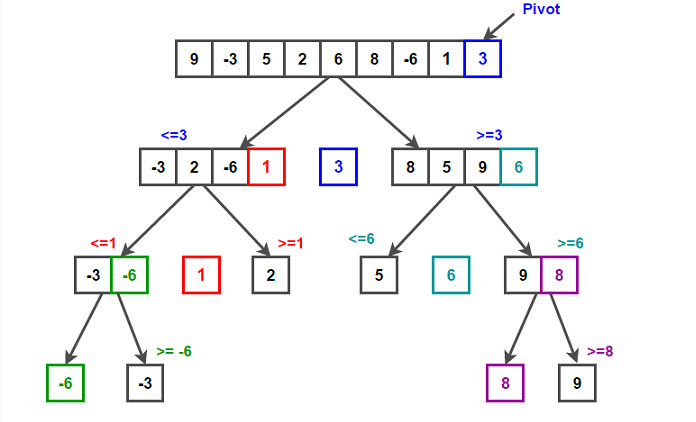
\includegraphics[scale=0.7]{1.jpg}\\
 \end{flushleft}
\begin{flushleft}
Сортировка слиянием — это эффективный алгоритм сортировки, обеспечивающий стабильную сортировку. Это означает, что если два элемента имеют одинаковое значение, они занимают то же относительное положение в отсортированной последовательности, что и во входных данных. Другими словами, в отсортированной последовательности сохраняется относительный порядок элементов с одинаковыми значениями. Сортировка слиянием — это сортировка сравнением, что означает, что она может сортировать любые входные данные, для которых меньше, чем отношение определено.
Сортировка слиянием — это Разделяй и властвуй алгоритм. Как и все алгоритмы «разделяй и властвуй», сортировка слиянием делит большой массив на два меньших подмассива, а затем рекурсивно сортирует подмассивы. По сути, весь процесс включает два этапа:
 \begin{itemize}
\item {Разделите несортированный массив на n подмассивы, каждый размером 1 (массив размера 1 считается отсортированным).}
\item {Неоднократно объединяйте подмассивы для создания новых отсортированных подмассивов до тех пор, пока не 1 остается подмассив, который будет нашим отсортированным массивом.}
\end{itemize}
 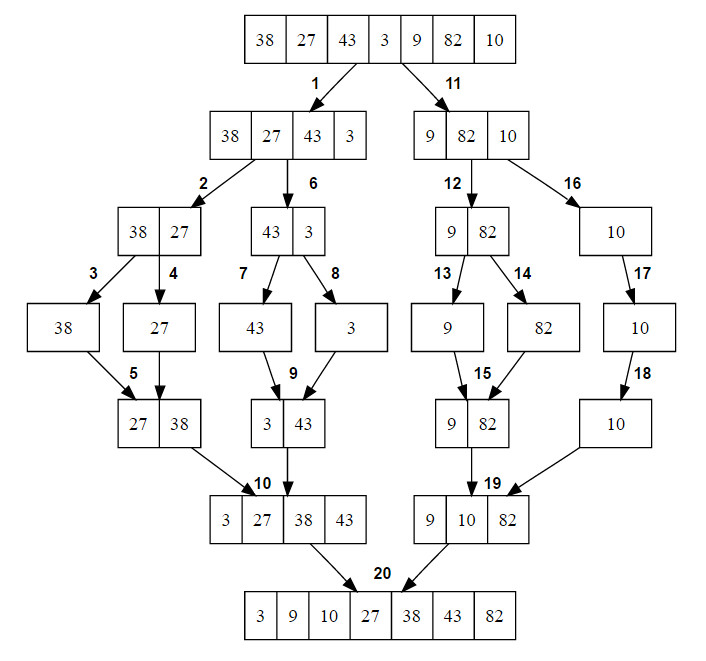
\includegraphics[scale=0.5]{4.jpg}\\
 \end{flushleft}
\begin{flushleft}
{\textbf{с. Изображение решения}}\\
Начальный экран\\
Вводим массивы чисел\\
 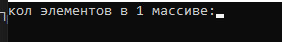
\includegraphics[scale=0.9]{2.jpg}\\
Вывод отсортированных массивов
 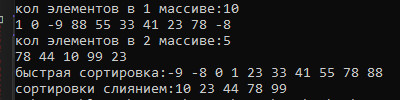
\includegraphics[scale=0.9]{3.jpg}\\

\end{flushleft}
\newpage
\begin{flushleft}
\textbf{{\Large Литература}}\\
\begin{enumerate}
\item \url{https://www.techiedelight.com/ru/quicksort/}
\item \url{https://www.techiedelight.com/ru/merge-sort/}
\end{enumerate}
\end{flushleft}
\end{document}